\chapter{Gegenüberstellung}

Anhand der unter \ref{qualitätsmetriken} erstellten Metriken sind die Frameworks GeoMesa, Postgres-XL und Rasdaman zu vergleichen.
Der Vergleich findet im Rahmen einer Nutzwertanalyse statt.
Hierbei werden keine Daten von durchgeführten Tests herangezogen, sondern es wird anhand der Spezifikation der einzelnen Frameworks untersucht.\\
%
Die drei Frameworks wurden aus der Tabelle der Abbildung \ref{fig:spatialdatabases} ausgewählt.
\begin{figure}
\centering
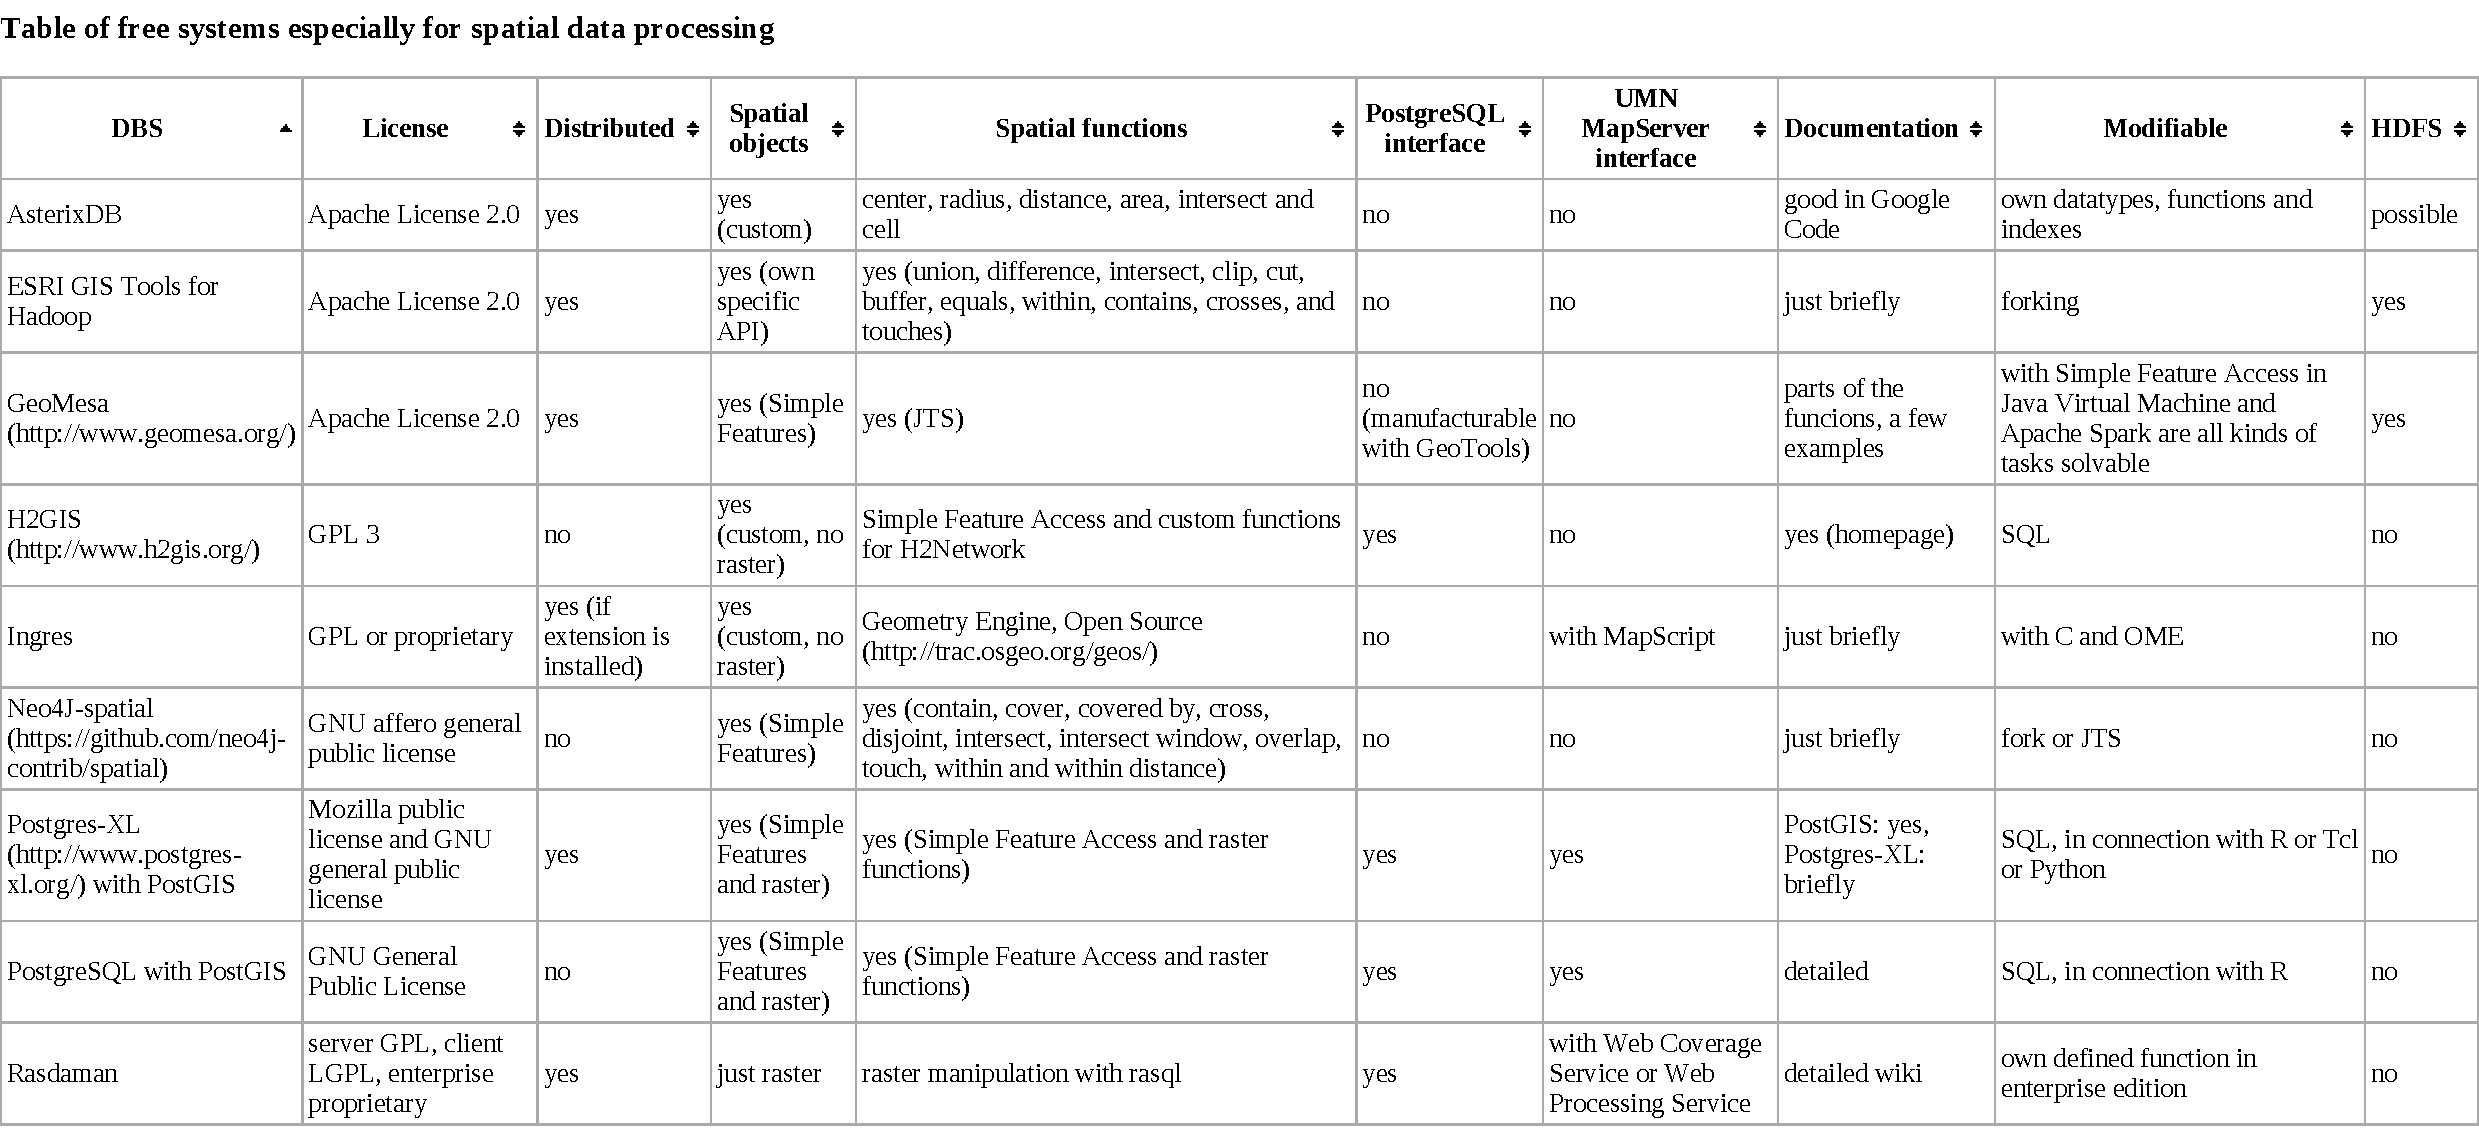
\includegraphics[width=\textwidth]{Abbildungen/table_spatialdatabases_13_2_15.pdf}
\caption[Übersicht relevanter GIS Frameworks]{Übersicht relevanter GIS Frameworks nach \cite{website:wiki-spatialdatabase} vom 2.2.2015}
\label{fig:spatialdatabases}
\end{figure}
Darin sind GIS zur räumlichen Datenverarbeitung mit wesentlichen Eigenschaften wie PostgreSQL Schnittstelle und räumliche Datentypen aufgelistet.
Entsprechend den Anforderungen wurden daraus drei Frameworks für die Nutzwertanalyse ausgewählt.\\
Abbildung \ref{fig:spatialdatabases} stammt von der Wikipedia Seite \url{https://en.wikipedia.org/wiki/Spatial_database} und ist wie unter \ref{aufrufe-spatialdatabases} beschrieben für Unternehmen interessant.
Der Autor erschuf die abgebildete Tabelle durch Recherche und stellte sie am 1.2.2015 in den Artikel.
In der Annahme, dass unternehmensbezogene Besucher der Seite fehlendes ergänzen oder falsches korrigieren würden, dient diese zur Auswahl geeigneter Frameworks.

%TODO: Nutzertanalyse: Struktur, Bewertungssystem, erklären

Tabelle \ref{table:Wertungsmassstab} zeigt die für die Nutzwertanalyse notwendige Wertung der einzelnen Metriken.
\begin{table}[h]
\centering
\begin{tabular}{l|l}
\textbf{Metrik} & \textbf{Gewichtung in \%} \\ \hline
%Richtigkeit & 10 \\ \hline
Interoperabilität & 30 \\ \hline
Funktionsumfang & 20 \\ \hline
%Fehlertoleranz & 8 \\ \hline
Dokumentation & 35 \\ \hline
%Zeitverhalten & 16 \\ \hline
Modifizierbarkeit & 15
\end{tabular}
\caption{Wertungsmaßstab der einzelnen Metriken}
\label{table:Wertungsmassstab}
\end{table}
Die Metriken Richtigkeit, Fehlertoleranz und Zeitverhalten werden nicht in die Analyse aufgenommen, da sie über die Spezifikation nicht belegbar sind.

Für jedes Framework wird eine Nutzwertanalyse durchgeführt und die dazugehörigen Tabellen dazu präsentiert.

Zu jeder Metrik wird der erreichte Wert, die ungewichtete Erfüllung, die gewichtete Erfüllung ein ein Kommentar angegeben.
Die ungewichtete Erfüllung bezieht sich auf den maximal zu erreichenden Wert der Metrik, die gewichtete Erfüllung dagegen auf die Erfüllung der Metrik in Bezug auf \ref{table:Wertungsmassstab}.
Die Kommentarspalte dient der Darstellung des Erreichens der Mindestanforderungen.
Der schlussendliche Nutzwert ergibt sich nach Zangemeister in \cite{website:nutzwertanalyse} aus der Summe der Produkte des Teilnutzens des jeweiligen Kriteriums mit der Gewichtung des Kriteriums.
Der Teilnutzen ist hier der Prozentuale Anteil der erreichten Punktzahl an der maximalen Punktzahl des Kriteriums.
Diese Prozentangabe wird als Wert mit der Gewichtung des Kriteriums multipliziert, woraus sich der Nutzwert für das Kriterium ergibt.
Die Summe aller dieser Teilnutzwerte ergibt den Nutzwert des Frameworks für den Anwendungsfall.

\section{GeoMesa}

\subsection{Interoperabilität}
\begin{description}
\item[PostgreSQL - 7] Scala  kann mit JDBC auf PostgreSQL zugreifen.
\item[\Gls{umn} - 0] \Gls{umn} bietet Accumulo nicht als Quelle an und GeoMesa biete keine \Gls{ogc} konformen Dienste wie WMS an.
\end{description}
Die Wertung für Interoperabilität ist somit 7 mit einer Erfüllung von 58\%.

\subsection{Funktionsumfang}
\begin{description}
\item[parallele Verarbeitung - 2] Verteilte Datenhaltung durch Accumulo auf \Gls{hdfs} und verteiltes sowie paralleles Rechnen mit beispielsweise Spark \cite{website:geomesaeclipse}
\item[gegrafische Datentypen - 12] Vollständige Datentypen aus Simple Feature Access. \cite{website:geomesaeclipse}
\item[Umrechnungsfunktionen - 10] Datenverarbeitung direkt in Spark mit GeoTools möglich. \cite{website:geotools-crs}
\item[Gruppierungsfunktionen - 7] Funktionale Verarbeitung mit Scala.
\item[Verschneidungsfunktionen - 3] \Gls{jts} stellt difference, union und symmetric difference zur Verfügung. \cite{website:jts-wikipedia}
\item[Overlayfunktionen - 2] \Gls{jts} stellt relate und overlay zur Verfügung.
\item[Filterfunktionen - 10] Räumliche Filterung ist  mit GeoTools möglich \cite{website:geotools-wiki}
\item[Schemaversionierung - 0] Accumulo erlaubt entsprechend des BigTable Ansatzes ein dynamisches Datenbankschema, jedoch ohne Versionierung. Einzig erzeugte Datentypen, bestehend aus Simple Features, können in GeoMesa als Konstrukt persistiert werden.
\end{description}
Daraus ergibt sich ein Wert von 48, was 79\% des maximal zu erreichenden Wertes ist.

\subsection{Dokumentation}
\begin{description}
\item[Installation - 1] Knappe Hinweise für GeoMesa auf \cite{website:geomesa-quickstart}, dagegen ausführliche Anleitungen für Accumulo auf \cite{website:accumulo-manual}.
\item[Zeitverhalten - 0] Keine Dokumentation vorhanden. %eventuell auf Postgis versus GeoMesa hinweisen
\item[Funktionsumfang - 1] Konkrete Funktionalität von GeoMesa nur grob auf \cite{website:geomesa-tutorials} angedeutet. MapReduce mit Accumulo ist ausführlich beschrieben. \cite{website:accumulo-manual}
\item[Interoperabilität - 1] Nicht explizit bei GeoMesa angegeben, aber Anbindungsmöglichkeiten mit Scala bzw. Java sind im allgemeinen ausführlich dokumentiert.
\item[Best Practise - 0] Keine Dokumentation vorhanden.
\item[Anpassbarkeit - 1] In \cite{website:geomesa-tutorials} sind einige Anregungen zu finden. Beispielsweise die Erzeugung eigener Schemabestandteile. \cite{website:geomesa-simplefeatures}
\end{description}
Das Qualitätskriterium Dokumentation wird für GeoMesa mit dem Wert 4, bzw. der Erfüllung von 31\%,  belegt.

\subsection{Modifizierbarkeit}
\begin{description}
\item[Verwendung eigener Datentypen - 0] Es sind eigene Schemas aber keine Datentypen erstellbar. \cite{website:geomesa-simplefeatures}
\item[Erstellung eigener Schnittstellen - 1] Indirekt über JDBC oder ODBC möglich.
\item[Erstellung eigener Funktionen - 1] Durch verschiedenste Frameworks zur Datenverarbeitung wie Spark beliebige Funktionen erstellbar.
\item[Verwendung der Programmiersprachen Scala oder R - 1] GeoMesa ist in Scala geschrieben und kann mit dieser verwendet werden. R kann über das Tool SparkR verwendet werden.
\item[Anlegen eigener Berechnungsvorgängen zur späteren Abarbeitung - 1] mit einer Vielzahl von Tools möglich wie Spark, \Gls{storm}, Pig und \Gls{cascading}.
\end{description}
Hier ist die Wertung 4 von 6 Punkten und damit 67\%.

\begin{table}[h!]
\centering
\small
\begin{tabular}{l|p{1.8cm}|c|p{3.1cm}|p{1.8cm}}
\textbf{Metrik} & \textbf{erreichter Wert} & \textbf{Erfüllung in \%} & \textbf{Kommentar} & \textbf{gewichteter Teilnutzen} \\ \hline
Interoperabilität & 7 & 58 & Implementationen notwendig & 17 \\ \hline
Funktionsumfang & 48 & 79 & meisten Funktionen nur mit Scala verfügbar & 16 \\ \hline
Dokumentation & 4 & 31 & zumeist ist auf Community zurückzugreifen & 11 \\ \hline
Modifizierbarkeit & 4 & 67 & mit Simple Features und Spark mächtige Problemlösungen erstellbar & 10 \\
\end{tabular}
\caption{Nutzwertanalyse GeoMesa}
\label{table:nutzwertanalyse-geomesa}
\end{table}
Der Nutzwert von GeoMesa ist nach Tabelle \ref{table:nutzwertanalyse-geomesa} 54.



\section{Postgres-XL}
\begin{table}[htp]
\centering
\small
\begin{tabular}{l|p{1.8cm}|c|p{3.1cm}|p{1.8cm}}
\textbf{Metrik} & \textbf{erreichter Wert} & \textbf{Erfüllung in \%} & \textbf{Kommentar} & \textbf{gewichteter Teilnutzen} \\ \hline
Interoperabilität & 12 & 100 & analog Ist-Stand & 30 \\ \hline
Funktionsumfang & 59 & 97 & Geostatistik und Versionierung nicht vorhanden & 19 \\ \hline
Dokumentation & 9 & 69 & Dokumentation zu PostGIS sehr gut, zu Postgres-XL grob & 24 \\ \hline
Modifizierbarkeit & 5 & 83 & meist eigenständige Programme notwendig & 13 \\
\end{tabular}
\caption{Nutzwertanalyse Postgres-XL}
\label{table:nutzwertanalyse-postgresxl}
\end{table}
Aus Tabelle \ref{table:nutzwertanalyse-postgresxl} ergibt sich ein Nutzwert von 86.
% Funktionsumfang 59
%parallele verarbeitung: 2 partitioning over nodes and MPP http://www.postgres-xl.org/overview/
%geografische Datentypen: 14 OGC Simple feature and raster http://postgis.net/docs/manual-2.1/using_postgis_dbmanagement.html#idp6871632
%umrechnung: 10 einfacher Funktionsaufruf http://postgis.net/docs/manual-2.1/UpdateGeometrySRID.html
%gruppierung: 10 in SQL eingebaut (OGC) http://postgis.net/docs/manual-2.1/using_postgis_dbmanagement.html
%verschneidung: 3 fct für intersetction, difference and symmetric difference http://postgis.net/docs/manual-2.1/reference.html
%overlay: 2 fct for relation, intersects http://postgis.net/docs/manual-2.1/reference.html
%geostatistic: 2 just simple interpolation to a point, possible with R or C++ and GDAL http://postgis.net/docs/manual-2.1/PostGIS_Special_Functions_Index.html
%filter: 10 much functions http://postgis.net/docs/manual-2.1/reference.html
%versioning: not build in, possible with tools

% Interoperabilität 12
%pgsql ja
%umn: als Datenquelle angebbar http://mapserver.org/mapfile/layer.html

% Dokumentation 9
%PostGIS: http://postgis.net/documentation
%postgres-xl: http://files.postgres-xl.org/documentation/
%installation: 1 briefly http://files.postgres-xl.org/documentation/installation.html
%Zeitverhalten: 0
%funktionsumfang: 2 Übersicht managing, allgemeine postgreSQL und PostGIS Doku http://files.postgres-xl.org/documentation/
%Interoperabilität: 2 verweis auf postgresql doku, API http://files.postgres-xl.org/documentation/client-interfaces.html
%best practise: 1 some hints http://files.postgres-xl.org/documentation/
%anpassbarkeit: 3 sql, tcl, perl, python http://files.postgres-xl.org/documentation/server-programming.html

% Modifizierbarkeit 5
%eigene Datentypen mit SQL
%Schnittstellen: indirekt: JDBC, pgadmin http://www.postgres-xl.org/faq/
%eigene Funktionen mit SQL
%Programmiersprachen: R definitiv, Scala indirekt über JDBC
%Batch-Vorgänge über Trigger oder über JDBC/ODBC funktionsuafrufe


\section{Rasdaman}
\begin{table}[htp]
\centering
\small
\begin{tabular}{l|p{1.8cm}|c|p{3.1cm}|p{1.8cm}}
\textbf{Metrik} & \textbf{erreichter Wert} & \textbf{Erfüllung in \%} & \textbf{Kommentar} & \textbf{gewichteter Teilnutzen} \\ \hline
Interoperabilität & 12 & 100 & UMN MapServer Schnittstelle nur indirekt vorhanden & 30 \\ \hline
Funktionsumfang & 12 & 20 & umfangreiche Rasterverarbeitung möglich & 4 \\ \hline
Dokumentation & 8 & 62 & mehrere Dokumente vorhanden & 22 \\ \hline
Modifizierbarkeit & 3 & 60 & einfache Java und C++ API & 9 \\
\end{tabular}
\caption{Nutzwertanalyse Rasdaman}
\label{table:nutzwertanalyse-rasdaman}
\end{table}
Aus Tabelle \ref{table:nutzwertanalyse-rasdaman} ergibt sich ein Nutzwert von 65.

% Funktionsumfang 12
%parallele Verarbeitung: 1 ja auf einer maschine http://www.rasdaman.org/wiki/Features
%geografische Datentypen: 4 nur raster und Punkte (als array DBMS sind arrays mit beliebig vielen Dimensionen verwendbar) http://www.rasdaman.org/wiki/Introduction
%umrechnung: 0 nur mit GDAL möglich und 2D arrays http://earthserver.eu/trac/wiki/DocumentationGDALrasdaman
%gruppierung: 0 http://rasdaman.org/browser/manuals_and_examples/manuals/doc-guides/ql-guide.pdf
%verschneidung: 1 einfache Array-Operationen http://rasdaman.org/browser/manuals_and_examples/manuals/doc-guides/ql-guide.pdf
%overlay: 1 einfache Array-Operationen http://rasdaman.org/browser/manuals_and_examples/manuals/doc-guides/ql-guide.pdf
%geostatistik: 0
%filter: 5 einfache Operationen (auch für array) http://rasdaman.org/browser/manuals_and_examples/manuals/doc-guides/ql-guide.pdf
%schemaversionierung: 0

%% Interoperabilität 12
%pgsql ja http://www.rasdaman.org/wiki/Features
%umn: per WCS, WPF

% Dokumentation 8
%installation: 1 eigene pdf's http://www.rasdaman.org/wiki/Documentation
%Zeitverhalten: 0
%funktionsumfang: 2 grob http://www.rasdaman.org/wiki/Features , ausführlicher in speziellen pdf wie http://rasdaman.org/browser/manuals_and_examples/manuals/doc-guides/ql-guide.pdf
%Interoperabilität: 3 für postgres und API http://rasdaman.org/browser/manuals_and_examples/manuals/doc-guides/ql-guide.pdf
%best practise: 1 hints file:///C:/Users/KJunghanns/Downloads/inst-guide.pdf
%anpassbarkeit: 1 aus context der pdfs

% Modifizierbarkeit 3
% keine eigenen datentypen 0
%Schnittstellen: mit Java und C++
%eigene Funktionen: über API, rasql nicht
%Programmiersprachen: Java, somit Scala, R NICHT
%keine batchvorgägnge